\documentclass[10pt, a4paper]{article}
    \usepackage{amsmath, amssymb, amsthm}
    \usepackage[margin=0.1in, landscape]{geometry}
    \usepackage{graphicx}
    \usepackage{verbatim}
    \usepackage{multicol}
    \DeclareMathOperator*{\argmax}{\arg\!\max}
    \usepackage[compact]{titlesec}
    \usepackage{transparent}
    \usepackage{eso-pic}
    \usepackage[nodisplayskipstretch]{setspace} \setstretch{1.5}
    \usepackage{etoolbox}
    \preto{\verbatim}{\edef\tempstretch{\baselinestretch}\par\setstretch{1}}
    \appto{\endverbatim}{\vspace{-\tempstretch\baselineskip}\vspace{\baselineskip}}
    \titlespacing*{\section}{0pt}{-5pt}{-3pt}
    \linespread{1.0}
    \setlength{\columnseprule}{0.4pt}
    \makeatletter
    \preto{\@verbatim}{\topsep=0pt \partopsep=0pt }
    \makeatother

\begin{document}
    \begin{multicols*}{1}
        \section*{Reinforcement Learning}
            \textbf{Def:} Use a MDP: set of states, set of actions, transition model, reward function and $\gamma$. Don't know transition or reward functions (learn them).\\
            \textbf{Passive Learning} Input is a policy, execute and learn the transitions and rewards.\\
            \textbf{Passive (Model):} Count outcomes $s'$ for each $s, a$, normalize to get transition model $X$. Discover $R(s, a, s')$ when we experience $(s, a, s')$.\\
            \textbf{Passive (Model Free):} Similar to the above but instead of calculating $E[X]$ from $P(X)$, it is calculated from the average of all of the samples.\\
            \textbf{Sample Evaluation:} Execute policy $n$ times from state $s$ and observe reward given. \\let $sample_i = R(s, \pi(s), s'_i) + \gamma V_k^\pi (s'_i)$ then $V_{k+1}^\pi \leftarrow \frac{1}{n} \sum\limits_i^n sample_i$\\
            \textbf{Temporal Difference Learning:} Update $V(s)$ each time we experience transition $(s, a, s', r)$. Let $sample = r + \gamma V^\pi (s')$ then $V^\pi(s) \leftarrow (1 - \alpha)V^\pi(s) + (\alpha) sample$\\
            \textbf{Active Reinforcement Learning:} Learner makes choices and learns optimal policy.\\
            \textbf{Q-Learning:} Learn $Q(s, a)$ as you go (off-policy learning). Receive a sample $(s, a, s', r)$ let $sample = r + \gamma \max\limits_{a'} Q(s', a')$ and update $Q(s, a) \leftarrow (1 - \alpha) Q(s, a) + (\alpha) sample$\\
            \textbf{Epsilon Greedy:} With probability $\epsilon$ act randomly, otherwise act on current policy.\\
            \textbf{Exploration Functions:} $f(\mu, n)$ Takes a value estimate, $\mu$, and visit count, $n$, and returns optimistic utility. Change $sample = r + \gamma \max\limits_{a'}f(Q(s', a'), N(s', a'))$\\
            \textbf{Regret:} $\Delta$ between your expected rewards while learning and the optimal rewards.\\
            \textbf{Approximate Q-Learning:} Represent states with features and weights. $Q(s, a) = \sum\limits_i w_i f_i(s, a)$ Update with $\delta = r + \gamma \max\limits_{a'} Q(s', a') - Q(s, a)$ and $Q(s, a) \leftarrow Q(s, a) + (\alpha) \delta$ and $w_i \leftarrow w_i + (\alpha) \delta f_i(s, a)$. Online least squares (adjust weights of active features).\\
            \textbf{Policy Search:} Learn policies that maximize rewards, not the values that predict them by hill climbing. (nudge feature weights up and down to see if improvement).
        \section*{Probability}
            \textbf{Rules:} Product: $P(y)P(x|y) = P(x, y)$ Chain: $P(x_{1:n}) = \prod\limits_i P(x_i | x_{1:i - 1})$\\ Bayes': $P(x|y) = \frac{P(y|x)P(x)}{P(y)}$ Independence: $x \!\perp\!\!\!\perp\! y \leftrightarrow P(x|y) = P(x) P(y)$\\
            \textbf{Conditional Independence:} $X \!\perp\!\!\!\perp\! Y | Z$ iff $\forall x, y, z: P(x,y|z) = P(x|z)P(y|z)$
        \section*{Markov Models}
            \textbf{Def:} Value of X at a given time is called the state.\\
            \textbf{Independence:} $X_{t + 1} \!\perp\!\!\!\perp\! X_{1:t-1} | X_{t} \implies P(X_{1:T}) = P(X_1) \prod\limits_{t=2}^T P(X_t | X_{t-1})$\\
            \textbf{Mini-Forward:} $P(X_t = x_t) = \sum\limits_{x_{t - 1}} P(x_{t - 1}, x_t) = \sum\limits_{x_{t - 1}} P(x_t | x_{t - 1}) P(x_{t - 1})$\\
            \textbf{HMMs:} Observable evidence variables $E_n$ for each $X_n$\\ $P(X_{1:n}, E_{1:n}) = P(X_1)P(E_1|X_1)\prod\limits_{i=2}P(X_i|X_{i-1})P(E_i|X_i)$\\
            \textbf{Computations:} Filtering $P(X_t | e_{1:t})$, Smoothing $P(X_t | e_{1:n}), n>t$, and Most Probable Explanation $x^*_{1:n} = \argmax_{x_{1:n}} P(x_{1:n} | e_{1:n})$\\
            \textbf{Online Belief Updates:} Time: $P(x_t|e_{1:t-1})=\sum\_{x_{t-1}}P(X_t|X_{t-1})P(X_{t-1}|e_{1:t-1})$ Observation: $P(X_t|e_{1:t})=P(e_t|X_t)P(X_t|e_{1:t-1})$ Update belief for state $X_t$ based on the previous evidence, then update on $e_t$\\
            \textbf{Forward Algorithm:} Combine both updates into a single one (time and observation). $P(x_t, e_{1:t}) = P(e_t|x_t) \sum\limits_{x_{t-1}} P(x_t | x_{t - 1}) P(x_{t-1}, e_{1:t-1})$ Time: $O(|X|^2)$ Space: $O(|X|)$\\
            \textbf{Particle Filtering:} Track samples of X, not all of the values. Elapse Time: $x' = sample(P(X' | x))$, Observe: $w(x) = P(e | x)$, Resample (w/ weights and w/ replacement)
        \section*{Bayes' Nets}
            \textbf{Dynamic Bayes Nets:} Abstraction of HMM, with multiple variables and inputs at once.\\
            \textbf{Probabilities:} $P(x_{1:n}) = \prod_{i=1} P(x_i | parents(X_i))$ Every BN represents a join distribution, but not every distribution can be represented by a specific BN. Size: $d^n$ where d is the dimension and n is the number of variables.\\
            \textbf{Causality:} Topology may encode structure but it really encodes conditional independence.\\
            \textbf{Independence in BN:} Given nodes $A,B\quad A \!\perp\!\!\!\perp\! B$ iff $\forall$ undirected paths between $A$ and $B$, there is an inactive triple in every path.\\
            \textbf{Inference by Enumeration:} Create one giant CPT with every single variable, and sum over the relevant conditions.\\
            \textbf{Variable Elimination (VE):} \\
            \begin{tabular}{l|c}
            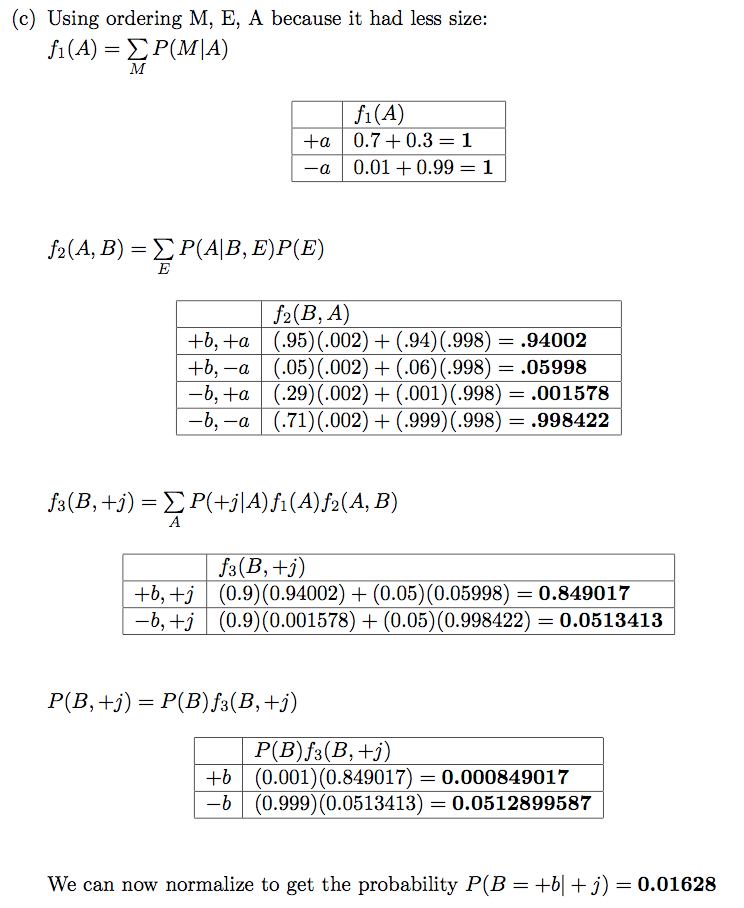
\includegraphics[height=230px]{VE.png} &  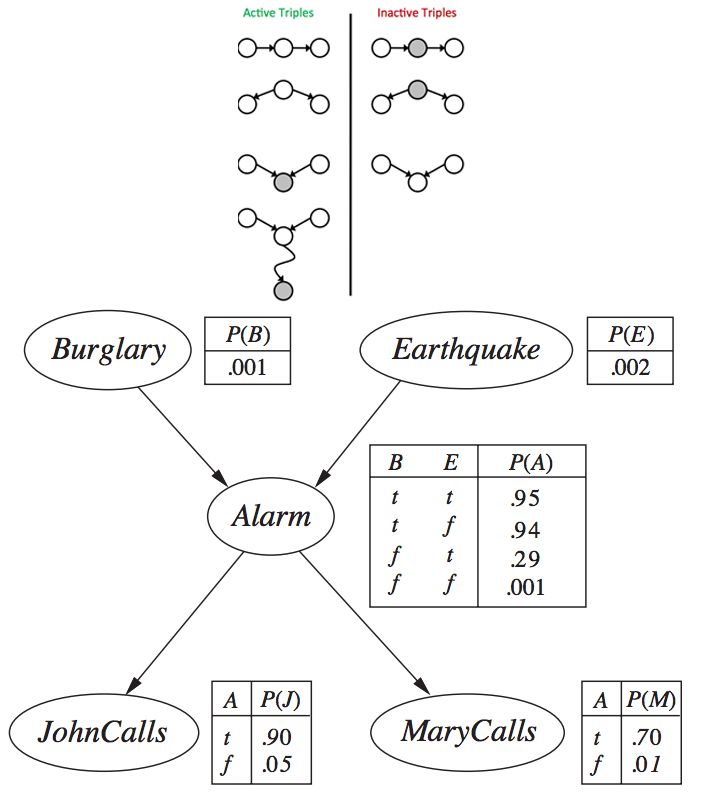
\includegraphics[height=230px]{graph2.png} \\
            \end{tabular}\\
            \textbf{VE Cont.:} NP-Hard, determined by size of largest factor (not always an efficient ordering).\\
            \textbf{Polytree} A directed graph with no undirected cycles (efficient ordering for VE). Choose a set of variables such that if removed only a polytree remains.\\
            \textbf{Expectation:} The expected outcome of the distribution given the observed data (the most likely). Requires uniform priors. \\
            \textbf{Maximum A Posteriori:} The best hypothesis that fits observed data. Arbitrary prior.\\
            \textbf{Bayesian Estimate:} Weighted combination of possibilities. Arbitrary Prior.\\
            \textbf{Prior:} Binary variable (Beta$(\alpha, \beta)$), discrete variable (Dirichlet)\\
            \textbf{Naive Bayes:} Features are independent given class: $P(X_{1:n} | Y) = \prod_i P(X_i | Y)$\\
            \textbf{Laplace Smoothing:} Pretend you saw every outcome K (1) more than you actually did.\\
            \textbf{Expectation Maximization:} Randomly initialize K distributions. Compute the likelihood for each sample to be in each distribution and assign it to the most likely. Compute the MLE for the parameters of each distributions given the samples in it. Repeat.\\
            \textbf{Learning Structure:} Search through the space of possible network structures. For each structure, learn the parameters and pick the one that fits observed data best. Use local search (to converge quickly) and add penalty term (regularization) proportional to model complexity.\\
            \textbf{Bayesian Information Criterion:} $score = P(Data | BN) - penalty$ where $penalty =\alpha 0.5 * (|parameters|) * \log (|Data|)$. Never test with training data (k-fold cross validation).
            \newpage
        \section*{Markov Decision Processes}
            \textbf{Def:} states, actions, Transition $T(s, a, s')$ or $P(s' | s, a)$, Reward $R(s, a, s')$ or $R(s)$\\
            \textbf{Policy:} $\pi^{*}: S \to A$, gives an optimal action for all states\\
            \textbf{Discounting:} Each time a level is descended multiply by another factor of $\gamma$\\
            \textbf{Bellman Equations:} $V^*(s) = \max\limits_{a} Q^*(s, a) = $ utility starting in s and then acting optimally, $Q^*(s, a) = \sum_{s'} T(s, a, s') [R(s, a, s') + \gamma V^*(s')] = $ utility starting after taking action a in s then acting optimally\\
            \textbf{Value Iteration:} $V_0(s) = 0$, given $V_k(s)$ simultaneously solve one ply of expectimax from each state: $V_{k + 1}(s) \gets \sum_{s'} T(s, a, s') [R(s, a, s') + \gamma V_k^*(s')]$ with Time: $O(|S|^2|A|)$\\
            \textbf{Policy Extraction:} Given the optimal values, $V^*(s)$, $\pi^*(s) = \argmax\limits_{a} Q^*(s, a)$\\
            \textbf{Problems:} Slow, max at each state rarely changes and the policy often converges long before the values do\\
            \textbf{Asynchronous Value Iteration:} Not essential to back up all states in each iteration as long as no state is starved. Backup with a heap of states ordered by the expected change in value (prefer backing a state whose successors had most change\\
            \textbf{Policy Evaluation:} compute the utility of a state s under a fixed policy
            \textbf{Policy Iteration:} Initialize $\pi(s)$ to random actions, calculate utilities of $\pi$ at each s using a nested loop, update policy using one-step look-ahead to see what's the best action I could execute, assuming I then follow $\pi(s)$\\
            \hspace*{5 mm}Initialize $\pi_i(s)$ to random actions and $i = 0$. Repeat:\\
            \hspace*{10 mm}Step 1: Policy Evaluation:\\
            \hspace*{15 mm}Initialize $k = 0$ and for each s, $V_0^\pi(s) = 0$ and repeat until $V^\pi$ converges:\\
            \hspace*{20 mm}For each s $V_{k + 1}^{\pi_i}(s) \gets \sum_{s'} T(s, \pi_i(s), s') [R(s, \pi_i(s), s') + \gamma V_k^{\pi_i}(s')]$\\
            \hspace*{15 mm}$k++$\\
            \hspace*{10 mm}Step 2: Policy Improvement:\\
            \hspace*{15 mm}For each s, $\pi_{i + 1}(s) = \argmax\limits_{a} \sum_{s'} T(s, a, s') [R(s, a, s') + \gamma V^{\pi_i}(s')]$\\
            \hspace*{15 mm}If $\pi_i == \pi_{i + 1}$, then it is optimal\\
            \hspace*{15 mm}Else let $i++$
        \section*{Adversarial Search}
            \textbf{Minimax:} The opitmal utility with a rational adversary, Time: O($b^m$), Space: O($bm$)\\
            \textbf{Pruning:} $\alpha$ is Max's best choise on a path to root. If the best value becomes worse than $\alpha$, no point in exploring children. Similiar for $\beta$. Time: O($b^{m / 2}$)
            \begin{verbatim}
def value(state, agent, alpha, beta):
    for each successor of state:
        if agent == 0:
            v = max(v, value(successor, agent + 1, alpha, beta))
            if v >= beta: return v
            alpha = max(alpha, v)
        else:
            v = min(v, value(successor, agent + 1, alpha, beta))
            if v <= alpha: return v
            beta = min(beta, v)
    return v
            \end{verbatim}
            \textbf{Expectimax:} Instead of the min value being chosen, the expected value for that state is returned: $\sum_{i} [value(successor_{i}) * P(successor_{i})]$\\
            \textbf{Utility:} Function from state to real numbers that describe an agent's preferences
        \section*{Agents}
            \textbf{Rational:} Maximally achieving goals (actions that maximize utility function) \\
            \textbf{Reflex Based:} Chooses action based on current percept (no future consideration)\\
            \textbf{Goal Based:} Chooses action based on consequences (model of how the world reacts)\\
            \textbf{Utility Based:} Goal based with trading off of multiple goals and uses probabilities
        \section*{Constraint Satisfaction Problems (CSPs)}
            \textbf{Def:} Goal test is a set of constraints over the state's variables $x_i$ $\in D_i\ or\ D$\\
            \textbf{Forward Checking:} Cross off values that violate a constraint when added to the existing assignment (Immediate neighbors and fail if the set of possible values is empty)\\
            \textbf{Arc Consistency:} An arc $X \to Y$ is consistent iff for every x in the tail there is some y in the head which could be assigned without violating a constraint\\
            \textbf{Constraint Propagation:} If X loses a value, neighbors of X need to be rechecked\\
            \textbf{Min Remaining Values:} Choose the variable with fewest legal values in its domain\\
            \textbf{Max Degree:} Choose the variable in the most constraints with remaining variables\\
            \textbf{Least Constraining Value:} Given a variable, assign a value that rules out the fewest values in remaining variables
        \section*{Stochastic Search}
            \textbf{Hill Climbing++ Restarts:} Generate random state when plateaued\\
            \textbf{Hill Climbing++ Walk:} With prob $p$ move to the neighbor with largest value, with $(1 - p)$ move to a random neighbor\\
            \textbf{Hill Climbing++ (Both):} Greedy move, random walk, or random restart\\
            \textbf{Simulated Annealing:} Pick a random neighbor and calculate the change in `energy' or objective function $\delta$, if it is positive then move to that state. Otherwise, move to this state with probability $e^\frac{\delta}{T}$ where T is decreased as the algorithm runs longer. High T = greater P(bad)
        \section*{Search}
            \textbf{Def:} Possible states, Successor function $f(n) \to$ ($n'$, action, cost), start and goal state\\
            \textbf{Complete:} Guaranteed to find a solution if one exists\\
            \textbf{Optimal:} Guaranteed to find the least cost path\\
            \textbf{Properties:} n$ =$ number of states, b$ =$ maximum branching factor, $C^*$$ =$ optimal cost, d$ =$ depth of shallowest solution, m$ =$ max depth, $\epsilon =$ min cost of all actions\\
            \textbf{Conformant Planning:} Set of actions that always work (sterilizing surgical gear)
        \section*{Blind Search}
            \textbf{DFS:} Fringe uses a Stack, complete iff finite, not optimal, time: O(b$^{m}$), space: O(bm)\\
            \textbf{BFS:} Fringe uses a Queue, complete, optimal (constant), time and space: O(b$^{d}$)\\
            \textbf{IDDFS:} Fringe uses a Stack, complete, optimal (constant), time: O(b$^{d}$), space: O(bm)
        \section*{Heuristic Search}
            \textbf{Admissible:} Always an underestimate to the true lowest cost\\
            \textbf{Consistent:} Always $h(n) <= h(n') + stepCost(n')$ where n' is a neighbor of n\\
            \textbf{Best First:} Fringe uses a PriorityQueue with cost fuction $f(n)$ for each node\\
            \textbf{Uniform Cost:} Best First with $f(n)=$ sum of edge costs from  start to n (explores increasing contours), complete, optimal, time and space: O($b^{\frac{C^*}{\epsilon}}$)\\
            \textbf{Greedy:} Best First with $f(n)= h(n)$ (suboptimal goal is common)\\
            \textbf{A$^*$:} Best First with $f(n)= g(n) + h(n)$ with $g(n)=$ sum of costs from start to n\\
            \textbf{IDA$^*$:} Depth bound is now $F_{limit} = h(start)$, prune if $f(n) > F_{limit}$,\\ $F_{limit}' = min(pruned\ nodes)$, uses space of DFS, time depends on \# of unique F values\\
            \textbf{Beam:} Best First with $|Fringe| = K$, not complete, time: O($b^d$), space: O($b + K$)\\
            \textbf{Hill Climbing:} Always choose best child (Beam Search with K = 1)\\
            \textbf{Tabu:} Keep fixed length queue of states to not visit again (use with hill climbing)
    \end{multicols*}
\end{document}
